\documentclass[UTF8]{beamer}
\usefonttheme[onlymath]{serif}
\setbeamertemplate{navigation symbols}{}
\usetheme{CambridgeUS}
%\setbeamerfont{text}{family*={ptm}, shape=\upshape, series=\mdseries}

\title{Verifiable Delay Function}
\author{--}
\institute[SJTU]{Shanghai Jiao Tong University}

\usepackage{subfigure}

\newcommand{\Setup}{\textsf{\textit{Setup}}}
\newcommand{\Eval}{\textsf{\textit{Eval}}}
\newcommand{\Verify}{\textsf{\textit{Verify}}}
\newcommand{\SNKGen}{\textsf{\textit{SNKGen}}}
\newcommand{\SNKProve}{\textsf{\textit{SNKProve}}}
\newcommand{\SNKVerify}{\textsf{\textit{SNKVerify}}}
\newcommand{\IVCGen}{\textsf{\textit{IVCGen}}}
\newcommand{\IVCProve}{\textsf{\textit{IVCProve}}}
\newcommand{\IVCVerify}{\textsf{\textit{IVCVerify}}}
\newcommand{\Prime}{\textsf{\textit{Prime}}}

\newcommand{\pp}{\mathbf{pp}}
\newcommand{\poly}{\textsf{\textit{poly}}}
\newcommand{\negl}{\textsf{\textit{negl}}}

\newcommand{\cA}{\mathcal{A}}
\newcommand{\cB}{\mathcal{B}}
\newcommand{\cC}{\mathcal{C}}
\newcommand{\cD}{\mathcal{D}}
\newcommand{\cE}{\mathcal{E}}
\newcommand{\cF}{\mathcal{F}}
\newcommand{\cG}{\mathcal{G}}
\newcommand{\cH}{\mathcal{H}}
\newcommand{\cI}{\mathcal{I}}
\newcommand{\cJ}{\mathcal{J}}
\newcommand{\cK}{\mathcal{K}}
\newcommand{\cL}{\mathcal{L}}
\newcommand{\cM}{\mathcal{M}}
\newcommand{\cN}{\mathcal{N}}
\newcommand{\cO}{\mathcal{O}}
\newcommand{\cP}{\mathcal{P}}
\newcommand{\cQ}{\mathcal{Q}}
\newcommand{\cR}{\mathcal{R}}
\newcommand{\cS}{\mathcal{S}}
\newcommand{\cT}{\mathcal{T}}
\newcommand{\cU}{\mathcal{U}}
\newcommand{\cV}{\mathcal{V}}
\newcommand{\cW}{\mathcal{W}}
\newcommand{\cX}{\mathcal{X}}
\newcommand{\cY}{\mathcal{Y}}
\newcommand{\cZ}{\mathcal{Z}}

\newcommand{\bG}{\mathbb{G}}
\newcommand{\bN}{\mathbb{N}}
\newcommand{\bZ}{\mathbb{Z}}

\newcommand{\leftdollar}{\xleftarrow{\text{\tiny$\mathsf{\$}$}}}

\begin{document}
	\usebeamerfont{text}
	\begin{frame}
		\titlepage
	\end{frame}

	\begin{frame}{Time-lock puzzle}
		\begin{block}{Time-lock puzzle}
			The goal of time-lock puzzle is to ``encrypt" a message that cannot be decrypted by \textbf{anyone}, not even the sender, until a pre-determined amount of time has passed.
		\end{block}
		\begin{block}{Application scenario}
			\begin{figure}
				\centering
				\subfigure{
\includegraphics[width=3.5cm]{figure/auction.png}}
				\quad
				\subfigure{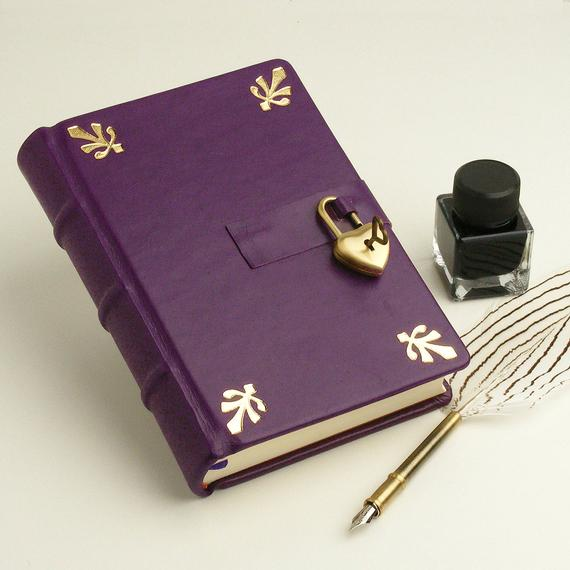
\includegraphics[width=3cm]{figure/secretdiary.jpg}}
				\quad
				\subfigure{
\includegraphics[width=3.5cm]{figure/secretkey.jpg}}
			\end{figure}
		\end{block}
	\end{frame}

	\begin{frame}{Time-lock puzzle}
		\begin{block}{Implementations of time-lock puzzle}
			There are two natural approaches to implementing:
			\begin{itemize}
				\item Using trusted agents who promise not to reveal the information until the pre-determined time.
				\item Using computational problems that cannot be solved in a certain amount of time.
			\end{itemize}
		\end{block}
		\begin{block}{Discussion}
			\begin{itemize}
				\item The agents must be trustworthy, otherwise the information may leak before the time.
				\item Users can use parallelism and designated hardware to accelerate the computational problems.
			\end{itemize}
		\end{block}
	\end{frame}

	\begin{frame}{Distributed solutions}
		\begin{block}{Secret sharing}
			The information can be separated into different agents using secret sharing. By this method, the assumption that agents are trusted can be mitigated.
			
			However, this method needs third parties and may suffers DoS attack.
		\end{block}
		\begin{block}{Computational methods}
			Computational methods is more reliable as its security relies on mathematics problems. Now there are many kinds of solutions such as memory-hard functions (MHFs), proof of sequential work (PoSW) and \textbf{verifiable delay functions (VDFs)}.
		\end{block}
	\end{frame}

	\begin{frame}
		\centering
		\huge Verifiable Delay Function
	\end{frame}

	\begin{frame}{Definition}
        \begin{block}{simple introduction}
            A VDF is a function whose evaluation requires running a given number of sequential steps, yet the result can be efficiently verified
        \end{block}
		\begin{block}{}
			A VDF $V=(\Setup,\Eval,\Verify)$ is a triple of algorithms as follows:
			\begin{itemize}
				\item $\Setup(\lambda, t)\to\pp=(ek,vk)$ is a randomized algorithm where $\lambda$ is security parameter, $t$ is desired puzzle difficulty and $\pp$ consists of an evaluation key $ek$ and a verification key $vk$.
				\item $\Eval(ek,x)\to(y,\pi)$ takes an input $x\in\cX$ and produces a \textbf{unique} output $y\in\cY$ and a (possible empty) proof $\pi$.
				\item $\Verify(vk,x,y,\pi)\to\{0,1\}$ is a deterministic algorithm.
			\end{itemize}
		\end{block}
	\end{frame}

	\begin{frame}{More about the definition}
		\begin{block}{}
			\begin{itemize}
				\item $\Setup$ might need randomness, leading to a scheme requiring a trusted setup.
				\item $\Eval$ may use random bits to generate $\pi$ but not to compute $y$.
				\item For all valid $\pp$ and all $x\in\cX$, $\Eval$ must run in parallel time $t$ with $\poly(\log(t),\lambda)$ processors.
				\item $\Verify$ must run in total time polynomial in $\log(t)$ and $\lambda$. Note that $\Verify$ is much faster than $\Eval$.
			\end{itemize}
		\end{block}
	\end{frame}

	\begin{frame}{Properties}
		\begin{block}{Correctness}
			A VDF $V$ is correct if for all $\lambda, t$, parameters $(ek,vk)\leftdollar\Setup(\lambda,t)$, and all $x\in\cX$, if $(y,\pi)\gets\Eval(ek,x)$ then $\Verify(vk,x,y,\pi)=1$
		\end{block}
		\begin{block}{Soundness}
			A VDF is sound if for all algorithm $\cA$ that run in time $O(\poly(t,\lambda))$
			\begin{equation*}
				\Pr\left[
				\begin{aligned}
					&\Verify(vk,x,y,\pi)=1\\
					&y\neq\Eval(ek,x)
				\end{aligned}
				~~\left|~~
				\begin{aligned}
					&\pp=(ek,vk)\leftdollar\Setup(\lambda, t)\\
					&(x,y,\pi)\gets\cA(\lambda,\pp,t)
				\end{aligned}
				\right.\right]=\negl(\lambda)
			\end{equation*}
		\end{block}
	\end{frame}

	\begin{frame}{Properties}
		\begin{figure}[h]
			\centering
			\begin{tabular}{|l|}
				\hline
				$\pp\leftdollar\Setup(\lambda,t)$\\
				$L\gets\cA_0(\lambda,\pp,t)$\\
				$x\leftdollar\cX$\\
				$y_\cA\gets\cA_1(L,\pp,x)$\\
				\hline
			\end{tabular}
		\end{figure}
		\begin{block}{}
			The sequentiality game is applied to an adversary $\cA:=(\cA_0,\cA_1)$. The adversary wins the game if $y_\cA=y$ where $(y,\pi):=\Eval(\pp,x)$.
		\end{block}
		\begin{block}{Sequentiality}
			For functions $\sigma(t)$ and $p(t)$, the VDF is $(p,\sigma)$-sequential if \textbf{no} pair of randomized algorithms $\cA_0$, which runs in total time $O(\poly(t,\lambda))$ and $\cA_1$ which runs in parallel time $\sigma(t)$ on at most $p(t)$ processors, can win the sequential game with probability greater than $\negl(\lambda)$
		\end{block}
	\end{frame}

	\begin{frame}{Some discussion}
		\begin{itemize}
			\item $t$ must be sub-exponential in $\lambda$.
			\item [-] The reason is that the adversary can run in time at least $t$, if $t$ is exponential in $\lambda$, then the adversary might be able to break the underlying computational security assumption.
			\item Parallelism in $\Eval$.
			\item [-] For a decodable VDF it is necessary that $|\cY|>\poly(t)$, and thus the challenge inputs to $\Eval$ have size $\poly(\log(t))$. Therefore, the algorithm $\Eval$ has up to $\poly(\log(t))$ parallelism.
			\item $\sigma$-sequentiality implies that min-entropy is $\Omega(\log(\lambda))$
			\item [-] If $t$ is sub-exponential in $\lambda$, then the output has $o(\lambda)$ min-entropy.
		\end{itemize}
	\end{frame}

	\begin{frame}{Value of $\sigma(t)$}
		\begin{itemize}
			\item Value of $\sigma(t)$.
			\item [-] Any candidate construction trivially satisfies $\sigma(t)$-sequentiality for some $\sigma$ (e.g. $\sigma(t)=0$). Security becomes more meaningful as $\sigma(t)\to t$. No construction can obtain $\sigma(t)=t$ by $\Eval$ design.
			\item [-] An almost-perfect VDF would achieve $\sigma(t)=t-o(t)$ sequentiality. $\sigma(t)=t-\epsilon t$ sequentiality for small $\epsilon$ is sufficient for most applications.
		\end{itemize}
	\end{frame}

	\begin{frame}{Weaker VDFs}
		\begin{block}{}
			For small values of $t$, it may be practical for anyone to use up to $O(t)$ parallelism. So a weaker variant of VDF allows additional parallelism in $\Eval$.
		\end{block}
		\begin{block}{Weaker VDF}
			A VDF $V=(\Setup,\Eval,\Verify)$ is a weak-VDF if it satisfies VDF definitions with exception that $\Eval$ is allowed up to $\poly(t,\lambda)$ parallelism.
		\end{block}
		\begin{block}{}
			Note that $(p,\sigma)$-sequentiality can only be meaningful for a weak-VDF if $\Eval$ is allowed strictly less than $p(t)$ parallelism, otherwise the honest computation of $\Eval$ would have more parallelism than adversary.
		\end{block}
	\end{frame}

	\begin{frame}
		\centering
		\huge Construction of VDFs
	\end{frame}

	\begin{frame}{Sequential function}
		\begin{block}{$(t,\epsilon)$-Sequential function}
			$f:\cX\to\cY$ is a $(t,\epsilon)$-sequential function if for $\lambda=O(\log(|\cX|))$, the following conditions hold:
			\begin{itemize}
				\item There exists an algorithm that for all $x\in\cX$ evaluates $f$ in parallel time $t$ using $\poly(\log(t),\lambda)$ processors.
				\item For all $\cA$ that run in parallel time strictly less than $(1-\epsilon)\cdot t$ with $\poly(t,\lambda)$ processors:
				\begin{equation*}
					\Pr\left[
					y_\cA=f(x)
					~\left|~
					y_\cA\gets\cA(\lambda,x), x\leftdollar\cX
					\right.\right]<\negl(\lambda)
				\end{equation*}
			\end{itemize}
		\end{block}
	\end{frame}

	\begin{frame}{Iterated Sequential Function}
		\begin{block}{Iterated Sequential Function}
			Let $g:\cX\to\cX$ be a function which satisfies $(t,\epsilon)$-sequentiality. A function $f:\bN\times\cX\to\cX$ defined as $f(k,x)=g^{(k)}(x)=\underbrace{g\circ g\circ\cdots\circ g}_{k~\text{times}}$ is called an iterated sequential function if for all $k=2^{o(\lambda)}$, the function $h:\cX\to\cX$ such that $h(x)=f(k,x)$ is $(k\cdot t,\epsilon)$-sequential.
		\end{block}
		\begin{block}{Instances}
			\begin{itemize}
				\item A chain of a secure hash function (like SHA-256).
				\item Exponentiation in a finite group of unknown order, the round function is squaring in the group.
			\end{itemize}
		\end{block}
	\end{frame}

	\begin{frame}{Iterated Sequential Function}
		\begin{block}{Assumption}
			For all $\lambda\in\bN$, there exists an $\epsilon,t$ with $t=\poly(\lambda)$ and a function $g_\lambda:\cX\to \cX~s.t.~\log(|\cX|)=\lambda$ and $\cX$ can be sampled in time $\poly(\lambda)$ and $g_\lambda$ is a $(t,\epsilon)$-sequential function, and the function $f:\bN\times\cX\to\cX$ with round function $g_\lambda$ is an iterated sequential function.
		\end{block}
		\begin{block}{}
			\begin{itemize}
				\item [-] An iterated sequential function is sequential by definition and the trivial function uses only $\poly(\lambda)$ parallelism.
				\item [-] However, the fastest generic verification is to simply recomputes the function, which do not satisfy the efficient verification requirement of VDF.
			\end{itemize}
		\end{block}
	\end{frame}

	\begin{frame}{SNARK}
		\begin{block}{SNARK}
			Let $\cL$ denote an NP language with relation $R_{\cL}$, where $x\in\cL$ iff $\exists w~R_{\cL}(x,w)=1$. A SNARK system for $R_{\cL}$ is a triple of polynomial time algorithms $(\SNKGen,\SNKProve,\SNKVerify)$ that satisfy the following properties:
		\end{block}
		\begin{block}{Completeness}
			$\forall(x.w)\in R_{\cL}$,
			\begin{equation*}
				\Pr\left[
				\SNKVerify(vk,x,\pi)=0
				~~\left|~~
				\begin{aligned}
					&(vk,ek)\leftdollar\SNKGen(1^\lambda)\\
					&\pi\gets\SNKProve(ek,x,w)
				\end{aligned}
				\right.\right]=0
			\end{equation*}
		\end{block}
		\begin{block}{Succinctness}
			The length of a proof and complexity of $\SNKVerify$ is bounded by $\poly(\lambda,\log(|y|+|w|))$.
		\end{block}
	\end{frame}

	\begin{frame}{SNARK}
		\begin{block}{Knowledge extraction}
			For all adversaries $\cA$ running in time $2^{o(\lambda)}$, there exists an extractor $\cE_\cA$ running in time $2^{o(\lambda)}$ such that for all $\lambda\in\bN$ and all auxiliary inputs $z$ of size $\poly(\lambda)$:
			\begin{equation*}
				\Pr\left[
				\begin{aligned}
					\SNKVerify(vk,x,\pi)=1\\
					R_{\cL}(x,w)\neq1
				\end{aligned}
				~~\left|~~
				\begin{aligned}
					&(vk,ek)\leftdollar\SNKGen(1^\lambda)\\
					&(x,\pi)\gets\cA(z,ek)\\
					&w\gets\cE_\cA(z,ek)
				\end{aligned}
				\right.\right]<\negl(\lambda)
			\end{equation*}
		\end{block}
	\end{frame}

	\begin{frame}{Impractical VDF from SNARGs}
		\begin{block}{}
			Consider the following construction for a VDF from a $(t,\epsilon)$-sequential function $f$:
			\begin{itemize}
				\item Let $\pp=(ek,vk)=\SNKGen(\lambda)$ be the public parameter of a SNARG scheme for proving membership in the language of pairs $(x,y)$ such that $f(x)=y$.
				\item On input $x\in\cX$, the $\Eval$ computes $y=f(x)$ and a succinct argument $\pi=\SNKProve(ek,(x,y),\bot)$, and outputs $((x,y),\pi)$.
				\item On input $((x,y),\pi)$, the verifier checks $y=f(x)$ by checking $\SNKVerify(vk,(x,y),\pi)=1$
			\end{itemize}
		\end{block}
		\begin{block}{Downsides}
			\begin{itemize}
				\item Computing a SNARG is more than $100000$ times more expensive than evaluating the underlying computation.
				\item The construction does not come asymptotically close to the sequentiality of the underlying computation $f$.
			\end{itemize}
		\end{block}
	\end{frame}

	\begin{frame}{Incremental Verifiable Computation (IVC)}
		\begin{block}{IVC}
			The basic idea of IVC is that for every step of computation, a prover can produce a proof of current state of computation. This proof is updated after every step of the computation to produce a new proof.
		\end{block}
		\begin{block}{Properties}
			\begin{itemize}
				\item The complexity of each proof in proof size and verification cost is bounded by $\poly(\lambda)$ for any sub-exponential length computation.
				\item The complexity of updating the proof is independent of the total length of the computation.
			\end{itemize}
		\end{block}
	\end{frame}

	\begin{frame}{Tight IVC for iterated sequential functions}
		\begin{block}{Tight IVC}
			Let $f_\lambda:\bN\times\cX\to\cX$ be an iterated sequential function with round function $g_\lambda$ having $(t,\epsilon)$-sequentiality. An IVC system for $f_\lambda$ is a triple of polynomial time algorithms ($\IVCGen,\IVCProve,\IVCVerify$) that satisfy the following properties:
		\end{block}
		\begin{block}{Completeness}
			$\forall x\in\cX$,
			\begin{equation*}
				\Pr\left[
				\IVCVerify(vk,x,y,k,\pi)=1
				~~\left|~~
				\begin{aligned}
					&(vk,ek)\leftdollar\IVCGen(\lambda,f)\\
					&(y,\pi)\gets\IVCProve(ek,k,x)
				\end{aligned}
				\right.\right]=1
			\end{equation*}
		\end{block}
		\begin{block}{Succinctness}
			The length of a proof and the complexity of $\SNKVerify$ is bounded by $\poly(\lambda,\log(k\cdot t))$
		\end{block}
	\end{frame}

	\begin{frame}{Tight IVC}
		\begin{block}{Soundness}
			For all algorithms $\cA$ running in time $2^{o(\lambda)}$
			\begin{equation*}
				\Pr\left[
				\begin{aligned}
					\IVCVerify(vk,x,y,k,\pi)\\
					f(k,x)\neq y
				\end{aligned}
				~~\left|~~
				\begin{aligned}
					&(vk,ek)\leftdollar\IVCGen(\lambda,f)\\
					&(x,y,k,\pi)\gets\cA(\lambda,vk,ek)
				\end{aligned}
				\right.\right]<\negl(\lambda)
			\end{equation*}
		\end{block}
		\begin{block}{Tight Incremental Proving}
			There exists a $k'$ such that for all $k\geq k'$ and $k=2^{o(\lambda)}$, $\IVCProve(ek,k,x)$ runs in parallel time $k\cdot t+O(1)$ using $\poly(\lambda,t)$-processors.
		\end{block}
		\begin{block}{Existance of tight IVC}
			Tight IVC can be constructed from existing SNARK constructions.
		\end{block}
	\end{frame}

	\begin{frame}{VDF construction from IVC}
		\begin{block}{}
			Let $f_\lambda:\bN\times\cX_\lambda\to\cX_\lambda$ defined by $f_\lambda(k,x)=g_\lambda^{(k)}(x)$, where $g_\lambda$ is a $(s,\epsilon)$-sequential function on an efficiently sampleable domain of size $O(2^\lambda)$. Given a tight IVC proof system $(\IVCGen,\IVCProve,\IVCVerify)$ for $f$, we can construct a VDF that satisfies $\sigma(t)$-sequentiality for $\sigma(t)=(1-\epsilon)\cdot t-O(1)$
		\end{block}
		\begin{block}{}
			\begin{itemize}
				\item $\Setup(\lambda,t)$: Let $f_\lambda$ be an iterated sequential function and $g_\lambda$ is the corresponding round function that is $(t,\epsilon)$ sequential. Run $(ek,vk)\leftdollar\IVCGen(\lambda,f_\lambda)$. Set $k$ to be the largest integer such that $\IVCProve(ek,k,x)$ takes time less than $t$. Output $\pp=((ek,k),vk)$.
				\item $\Eval((ek,k),x)$: Run $(y,\pi)\gets\IVCProve(ek,k,x)$, output $(y,\pi)$.
				\item $\Verify(vk,x,(y,\pi))$: Run and output $\IVCVerify(vk,x,y,k,\pi)$.
			\end{itemize}
		\end{block}
	\end{frame}

	\begin{frame}
		\centering
		\huge Practical VDF Construction
	\end{frame}

	\begin{frame}{VDF Construction}
		\begin{block}{Setup}
			The setup algorithm $\Setup(\lambda,T)$ outputs two objects:
			\begin{itemize}
				\item A finite abelian group $\bG$ of unknown order.
				\item An efficient computable hash function $H:\cX\to\bG$ that can be modeled as a random oracle.
			\end{itemize}
		\end{block}
		\begin{block}{Evaluation}
			The evaluation algorithm $\Eval(\pp,x)$ is defined as:
			\begin{itemize}
				\item compute $y\gets H(x)^{(2^T)}\in\bG$ by computing $T$ squaring in $\bG$ starting with $H(x)$.
				\item compute the proof $\pi$ as described later.
				\item output $(y,\pi)$.
			\end{itemize}
		\end{block}
	\end{frame}

	\begin{frame}{More about the construction}
		\begin{block}{}
			\begin{itemize}
				\item In practical one might set $T=2^{30}$.
				\item Let $g:=H(x)\in\bG$ be the basic element given as input to the VDF evaluator.
				\item Let $h:=y\in\bG$ be the purported output of the VDF, namely $h=g^{(2^T)}$.
				\item We need a succinct interactive argument for the language
				\begin{equation*}
					\cL_{EXP}:=\left\{
					(\bG,g,h,T):h=g^{(2^T)}~\text{in}~\bG
					\right\}.
				\end{equation*}
			\end{itemize}
		\end{block}
	\end{frame}

	\begin{frame}{VDF Construction (Wesolowski)}
		\begin{block}{Verification}
			Given a tuple $(\bG,g,h,T)$ as input, the prover and verifier run the following protocol to prove that $h=g^{(2^T)}$ in $\bG$. Let $\Prime(\lambda)$ be the set containing the first $2^\lambda$ primes.
			\begin{enumerate}
				\item [0.] The verifier checks that $g,h\in\bG$ and output $reject$ if not,
				\item [1.] The verifier sends to the prover a random prime $l$ sampled uniformly from $\Prime(\lambda)$,
				\item [2.] The prover computes $q,r\in\bZ$ such that $2^T=ql+r$ with $0\leq r<l$, and sends $\pi\gets g^q$ to the verifier,
				\item [3.] The verifier computes $r\gets 2^T\mod l$ and outputs $1$ if $\pi\in\bG$ and $h=\pi^lg^r$ in $\bG$.
			\end{enumerate}
		\end{block}
	\end{frame}

	\begin{frame}{VDF Construction (Wesolowski)}
		\begin{block}{Non-interactive variant}
			\begin{itemize}
				\item The prover first generates $l$ by hashing $(\bG,g,h,T)$ to an element of $\Prime(2\lambda)$.
				\item The prover computes $\pi\gets g^q$ as in step $2$ above, and outputs this $\pi\in\bG$ as the proof.
				\item The verifier computes $l$ as the same way as the prover and decides as step $3$ above.
			\end{itemize}
		\end{block}
	\end{frame}

	\begin{frame}{VDF Construction (Wesolowski)}
		\begin{block}{Verifier efficiency}
			The verifier needs to compute $r\gets 2^T\mod l$, which only takes $\log_2T$ multiplications in $\bZ_l$.
		\end{block}
		\begin{block}{Prover efficiency}
			Because $T$ is large, we cannot write out $q$ as an explicit integer exponent. However we can compute $\pi=g^q$ in at most $2T$ group operations and constant space using the long-division algorithm.
			\begin{enumerate}
				\item $\pi\gets1\in\bG, r\gets1\in\bZ$
				\item repeat $T$ times:
				\item [] $b\gets\lfloor2r/l\rfloor\in\{0,1\}~\text{and}~r\gets(2r\mod l)\in\{0,\dots,l-1\}$
				\item [] $\pi\gets\pi^2g^b\in\bG$
				\item output $\pi$ (this $\pi$ equals to $g^q$)
			\end{enumerate}
		\end{block}
	\end{frame}

	\begin{frame}{VDF construction (Pietrzak)}
		\begin{block}{Verification for $(\bG,g,h,T)\in\cL_{EXP}$}
			\begin{enumerate}
				\item [0.] The verifier checks that $g,h\in\bG$ and outputs $reject$ if not,
				\item [1.] If $T=1$ the verifier checks that $h=g^2$ in $\bG$, outputs $reject$ or $accept$, and terminate.
				\item [2.] If $T>1$ the prover and verifier do:
				\begin{enumerate}
					\item [a.] The prover computes $v\gets g^{(2^{T/2})}$ in $\bG$ and sends $v$ to the verifier. The verifier checks that $v\in\bG$ and outputs $reject$ and terminate if not.\\
					Next, the prover needs to convince the verifier that $h=v^{(2^{T/2})}$ and $v=g^{(2^{T/2})}$ which proves that $h=g^{(2^{T})}$. Since they have the same exponent, they can be verified simultaneously by checking a random linear combination, namely that
					$$v^rh=(g^rv)^{(2^{T/2})}\text{ for a random }r \text{ in } \{1,\dots,2^\lambda\}$$
					The verifier and prover do so as follows.
				\end{enumerate}
			\end{enumerate}
		\end{block}
	\end{frame}

	\begin{frame}{VDF construction (Pietrzak)}
		\begin{block}{Verification for $(\bG,g,h,T)\in\cL_{EXP}$}
			\begin{enumerate}
				\item [b.] The verifier sends to the prover a random $r$ in $\{1,\dots,2^\lambda\}$.
				\item [c.] Both the prover and verifier computes $g_1\gets g^rv$ and $h_1\gets v^rh$ in $\bG$.
				\item [d.] The prover and verifier recursively engage in an interactive proof that $(\bG,g_1,h_1,T/2)\in\cL_{EXP}$, namely that $h_1=g_1^{(2^{T/2})}$ in $\bG$.
			\end{enumerate}
		\end{block}
	\end{frame}

	\begin{frame}{VDF construction (Pietrzak)}
		\begin{block}{Non-interactive variant}
			The prover generates the challenge $r$ for every level of the recursion by hashing the quantities $(\bG,g,h,T,v)$ at that level, and appends $v$ to the overall proof $\pi$. Hence the overall proof $\pi$ contains $\log_2T$ elements in $\bG$.
		\end{block}
	\end{frame}

	\begin{frame}{VDF construction (Pietrzak)}
		\begin{block}{Verifier efficiency}
			At every level of recursion the verifier does two exponentiation in $\bG$ to compute $g_1,h_1$ for the next level. Hence the verifier needs $2\log_2T$ exponentiations in $\bG$.
		\end{block}
		\begin{block}{Prover efficiency}
			The prover needs to compute $v$ for every level of the recursion. We denote $v_i,r_i$ for the values of $v,r$ for the $i$-th recursion.
			\begin{equation*}
				\begin{aligned}
					v_1&=g^{(2^{T/2})}\\
					v_2&=g_1^{(2^{T/4})}=(g^{r_1}v_1)^{(2^{T/4})}=\left( g^{(2^{T/4})}\right)^{r_1}g^{(2^{3T/4})}\\
					v_3&=g_2^{(2^{T/8})}\\
					&=\text{ a power product of four elements } g^{(2^{T/8})}, g^{(2^{3T/8})}, g^{(2^{5T/8})}, g^{(2^{7T/8})}
				\end{aligned}
			\end{equation*}
		\end{block}
	\end{frame}

	\begin{frame}{VDF construction (Pietrzak)}
		\begin{block}{Prover efficiency}
			There exists an efficient way to compute these $v_i$.
			\begin{enumerate}
				\item [1.] When the prover first computes $h=g^{(2^T)}$, it stores $2^d$ group elements $g^{(2^{(i\cdot T/2^d)})}$ for $i=0,\dots,2^d-1$.
				\item [2.] These $2^d$ values will be used when the prover computes $v_1,\dots,v_d$, which takes about $2^d$ small exponentiation in $\bG$.
				\item [3.] The prover computes the remaining elements $v_{d+1},\dots,v_{\log T}$ by raising $g_{d+1},\dots,g_{\log T}$ to the appropriate exponents. This step takes a total of $T/2^d$ multiplications in $\bG$.
			\end{enumerate}
			Hence, the total time to compute these $v_i$ is about $2^d+T/2^d$, which is optimal when $d=\frac{1}{2}\log_2 T$. So the VDF output and the proof $\pi$ can be computed in total time approximately $T+2\sqrt{T}$.
		\end{block}
	\end{frame}

	\begin{frame}{Other constructions}
		\begin{block}{}
			content...
		\end{block}
	\end{frame}

\end{document} 